\documentclass[8pt,a4paper]{ctexart}
\usepackage[left=6mm,right=6mm,top=5.5mm,bottom=5.5mm]{geometry}
\usepackage{amsmath,amssymb}
\usepackage{multicol}
\usepackage[inline]{enumitem}
\usepackage[most]{tcolorbox}
\usepackage{xcolor}
\usepackage{titlesec}
\usepackage{setspace}
\usepackage{microtype}
\usepackage{tabularx}
\usepackage{array}
\usepackage{booktabs}
\usepackage{graphicx}
\usepackage{needspace}
\pagestyle{empty}
\setlength{\parindent}{0pt}
\setlength{\parskip}{0pt}
\setlength{\columnsep}{4pt}
\setlength{\columnseprule}{0.15pt}
\setlength{\multicolsep}{2pt}
\setlength{\premulticols}{0pt}
\setlength{\postmulticols}{0pt}
\setlist[itemize]{leftmargin=1.2em,itemsep=0pt,topsep=0pt,parsep=0pt,partopsep=0pt}
\setlist[enumerate]{leftmargin=1.4em,itemsep=0pt,topsep=0pt,parsep=0pt,partopsep=0pt}
\titlespacing*{\section}{0pt}{1pt}{1pt}
\renewcommand{\baselinestretch}{0.92}
\AtBeginDocument{\fontsize{5.55pt}{6.05pt}\selectfont}
\tcbset{
  colback=black!2,
  colframe=black!55,
  arc=0pt,
  boxrule=0.25pt,
  left=1pt,right=1pt,top=1pt,bottom=1pt,
  boxsep=0.4pt
}
\newcommand{\blk}[1]{%
  \par\needspace{2.2\baselineskip}%
  \vspace{1pt}\noindent
  \colorbox{black!10}{\parbox{\dimexpr\columnwidth-2\fboxsep\relax}{\textbf{#1}}}\par
  \vspace{1pt}}
\newcommand{\tightmath}[1]{\[
\vspace{-5pt}#1\vspace{-5pt}
\]}
\newcommand{\codebox}[1]{\begin{tcolorbox}#1\end{tcolorbox}}
\begin{document}
\raggedcolumns
\small
\begin{center}
{\bfseries 现代优化与智能计算 A4 双面速查}\\[-1pt]
\end{center}
\vspace{-3pt}
\begin{multicols*}{3}

\blk{遗传算法 GA：框架与高频点}
\textbf{思想：}在\textbf{编码空间}做选择/交叉/变异，在\textbf{解空间}算目标值与适值；基本流程：
\codebox{
编码$\leftrightarrow$解码 $\to$ 适值计算 $\to$ 选择 $\to$ 交叉 $\to$ 变异 $\to$ 下一代，直到终止。
}
\textbf{编码原则：}
\begin{itemize}
\item 完备性：所有解都能表示为染色体。
\item 健全性：染色体取值尽可能都对应合法解。
\item 非冗余性：解空间与编码空间尽可能一一对应。
\end{itemize}
\textbf{常见编码：}二进制、整数、顺序、实数。\\
\textbf{初始种群：}按编码随机生成，或用启发式生成。\\
\textbf{适值函数：}由目标函数经\textbf{适值标定}得到，直接影响收敛速度与是否易找到优解。\\
\textbf{约束处理：}
\begin{itemize}
\item 拒绝策略：丢弃不可行解；可行解少时难形成初始种群。
\item 修复策略：修回可行；易损失多样性。
\item 惩罚策略：$F'(x)=F(x)-\lambda P(x)$ 或等价最小化惩罚。
\end{itemize}
\textbf{典型参数：}$p_c=0.8\sim0.9$，$p_m<0.05$；可配\textbf{精英保留}，至少保留一个最优父代；GENITOR：父子合并后留最好者。\\
\textbf{编码适用：}二进制$\to$背包/部分实优化；整数$\to$离散决策；顺序$\to$指派/TSP/调度；实数$\to$连续优化。\\
\textbf{顺序口诀：}TSP 重相邻/先后$\Rightarrow$OX；指派重位值$\Rightarrow$CX；要合法又要映射$\Rightarrow$PMX。
\vspace{1pt}
\begin{center}
	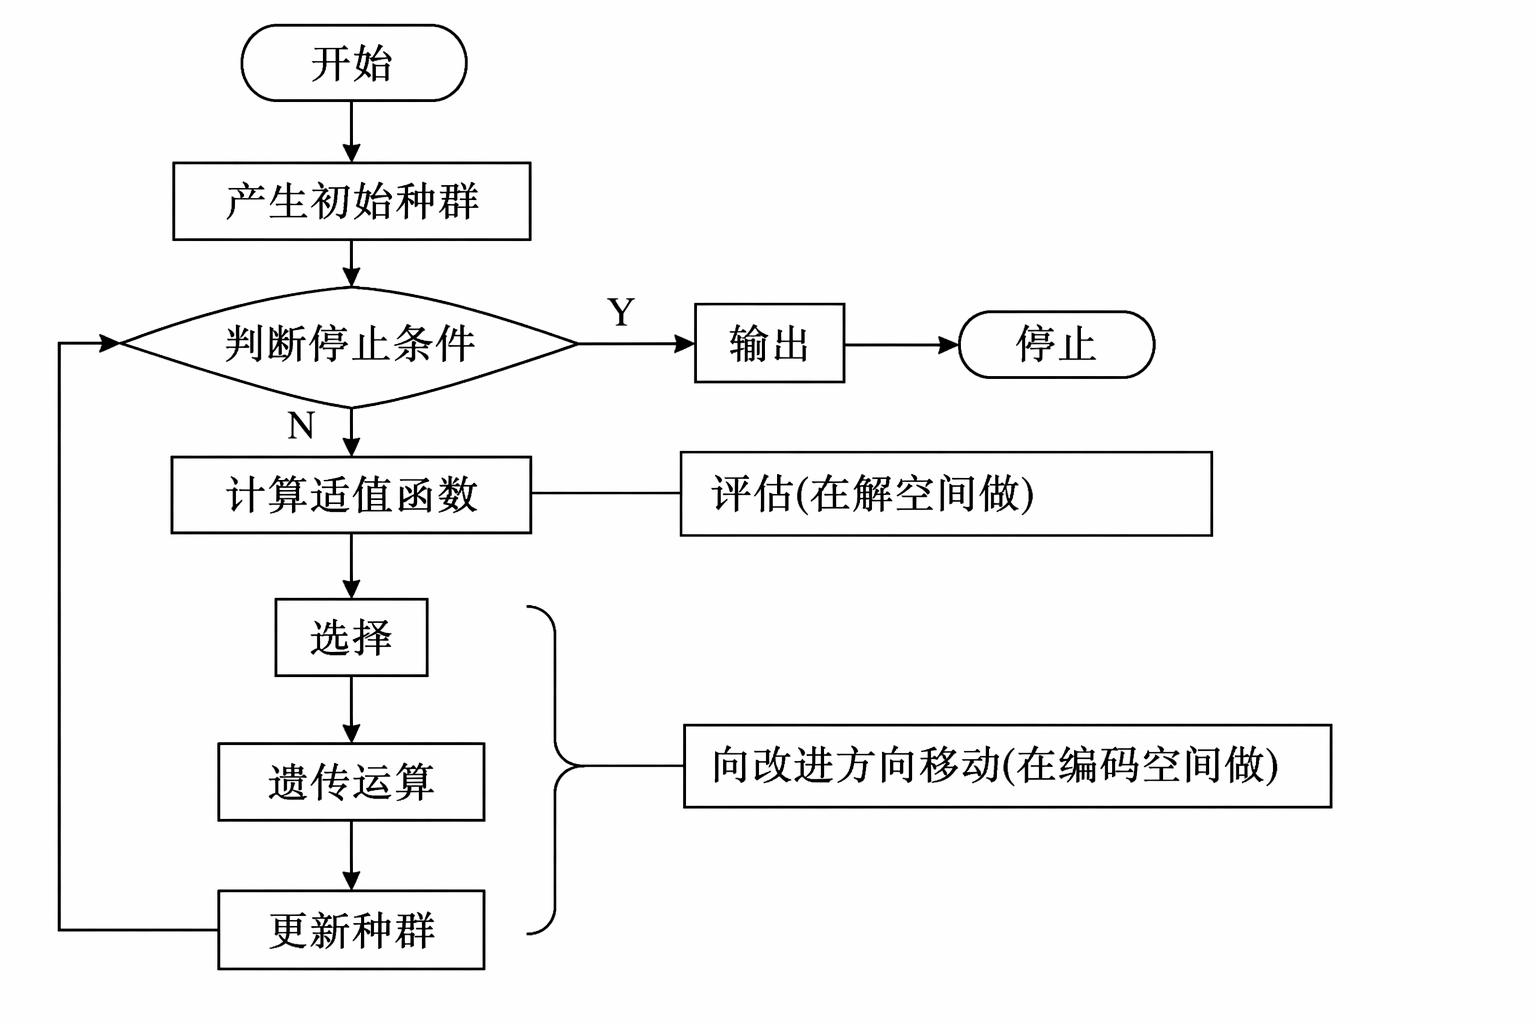
\includegraphics[width=0.92\columnwidth]{ga.png}
\end{center}
\vspace{-2pt}

\blk{GA：选择}
\textbf{选择压力：}最佳个体选中概率/平均个体选中概率；压力大则收敛快但易早熟。\\
\textbf{个体选择概率：}
\tightmath{P_i=\frac{f_i}{\sum_j f_j}}
\textbf{按排序适值分配：}先按好坏排序，再按名次给概率，避免个体适值尺度过于悬殊。\\
\textbf{方法：}
\begin{itemize}
\item \textbf{轮盘赌：}按累计概率采样，简单但方差较大。
\item \textbf{随机遍历抽样 SUS：}多个等距指针，方差小于轮盘赌。
\item \textbf{锦标赛：}随机抽若干个体，取其中最好者；实现简单、鲁棒。
\item 截断选择：只从前若干名中选，压力大。
\end{itemize}
\textbf{经验：}适值分布差异过大时优先排序选择/锦标赛；担心漂移时用 SUS。

\blk{GA：交叉}
\textbf{二进制/整数编码：}
\begin{itemize}
\item 单切点：选1点交换后段。
\item 双切点：选2点交换中段。
\item 均匀交叉：每一位按掩码从父母挑。
\end{itemize}
\textbf{顺序编码：}
\begin{itemize}
\item \textbf{PMX}：交换中段并建立映射，保合法排列。
\item 例：$P_1=21|345|67,\ P_2=43|125|76$；映射 $3\!\leftrightarrow\!1,\ 4\!\leftrightarrow\!2,\ 5\!\leftrightarrow\!5$，得 $C_1=43|125|67,\ C_2=21|345|76$。
\item \textbf{OX}：保留中段，其余按另一父代的相对顺序补齐；适合 TSP，相邻/先后关系保留较好。设 $P_1=34|125|67,\ P_2=12|345|67$，其中交叉段为第 3，4，5 位。则 $C_1=\_\,\_|125|\_\,\_$，去掉 $P_2$ 中已出现的 $1,2,5$，余下序列为 $3467$，按 OX 从交叉段右端后开始循环补齐空位（第 6,7,1,2 位），得 $C_1=34|125|67$；同理，$C_2=\_\,\_|345|\_\,\_$，去掉 $P_1$ 中已出现的 $3,4,5$，余下序列为 $1267$，按同样方式循环补齐，得 $C_2=12|345|76$。
\item \textbf{CX}：按循环传递位值；位值特征保留较好，适合指派。例：设 $P_1=(1\,2\,3\,4\,5\,6\,7),\ P_2=(4\,1\,2\,5\,7\,6\,3)$。从位置 1 开始构造循环：$1 \xrightarrow{P_2} 4 \xrightarrow{P_1} 4 \xrightarrow{P_2} 5 \xrightarrow{P_1} 5 \xrightarrow{P_2} 7 \xrightarrow{P_1} 7 \xrightarrow{P_2} 3 \xrightarrow{P_1} 3 \xrightarrow{P_2} 2 \xrightarrow{P_1} 2 \xrightarrow{P_2} 1$，故循环位置为 $(1,4,5,7,3,2)$，剩余位置为 $(6)$。子代 1 在循环位置取 $P_1$、其余位置取 $P_2$，得 $C_1=(1\,2\,3\,4\,5\,6\,7)$；子代 2 在循环位置取 $P_2$、其余位置取 $P_1$，得 $C_2=(4\,1\,2\,5\,7\,6\,3)$。
\end{itemize}
\textbf{实数编码：}
\begin{itemize}
\item 离散交叉：$z_i=x_i$ or $y_i$。
\item 线性交叉：$z_i=a x_i+(1-a)y_i,\ 0\le a\le1$。
\end{itemize}

\blk{GA：变异与流程伪代码}
\textbf{变异：}
\begin{itemize}
\item 二进制/整数：位变异。
\item 顺序：插入、交换、颠倒。
\item 实数：值变异。
\end{itemize}
\codebox{
\textbf{GA伪代码}\\
1.\ 初始化种群$P$；解码并算适值。\\
2.\ \textbf{while} 未满足终止条件 \textbf{do}\\
\quad 选择父代；按概率做交叉得子代；按概率变异；\\
\quad 解码并计算子代适值；按生存者选择形成下一代；\\
3.\ 输出最优个体/最优解。
}
\textbf{终止条件：}最大代数、最优值稳定、达到阈值。\\
\textbf{优缺点：}全局性强、并行性好、对导数不敏感；但参数多、编码依赖强、易早熟。

\blk{GA：模式/模板定理}
\textbf{模板} $s$：长度为 $l(s)$，阶数为 $K(s)$。模板中“\#”表示通配。\\
\textbf{引理1（正比选择）：}
\tightmath{E[s,t+1]=f(s,t)\,N(s,t)}
其中 $f(s,t)$ 为模板平均适值/群体平均适值。\\
\textbf{引理2（交叉后仍保模板下界）：}
\tightmath{P(s,t+1)\ge 1-\frac{p_c\,l(s)}{n-1}\,[1-P(s,t)]}
\textbf{引理3（变异后仍保模板下界）：}
\tightmath{P(s,t+1)\ge 1-p_m K(s)}
\textbf{模式定理：}
\tightmath{
\begin{aligned}
E[m(s,t+1)]\gtrsim\;&m(s,t)\frac{\bar f_s}{\bar f}\\
&\times\left(1-\frac{p_c\,l(s)}{n-1}-p_mK(s)\right)
\end{aligned}}
\textbf{结论：}短定义长度、低阶、平均适值高的模板会指数级增长，称\textbf{积木块假设}。

\blk{GA：Pr\"ufer数编解码}
\textbf{用途：}常用于最小生成树编码；对 $n$ 个节点，无向生成树个数与 Pr\"ufer 数个数均为 $n^{\,n-2}$，因此可实现解空间与编码空间一一对应，且交叉、变异后仍易保持合法性。编码：反复取\textbf{标号最小的叶子}，把与其相连的节点编号记入序列，再删去该叶子，直到只剩一条边；解码：对 Pr\"ufer 数中各元素统计出现次数，每次取\textbf{当前最小且未在序列中出现的节点}与序列首元素相连，删去该首元素并更新计数，最后连接剩余两个节点。例：树边集为 $(1,2),(2,3),(2,5),(4,5)$，编码时依次删叶子 $1,3,2$，得到 Pr\"ufer 数 $(2,2,5)$；反过来对 $(2,2,5)$ 解码：当前未出现最小点为 $1$，连边 $(1,2)$；删去首个 $2$ 后未出现最小点为 $3$，连边 $(3,2)$；删去首个 $2$ 后未出现最小点为 $2$，连边 $(2,5)$；最后剩余 $4,5$，连边 $(4,5)$，故恢复生成树边集为 $(1,2),(2,3),(2,5),(4,5)$。

\blk{GA：适值函数标定}
\textbf{作用：}把目标函数值变换为适值，使之适合选择操作；最大化问题可直接取 $f(x)=F(x)$，最小化问题常作非负变换，如 $f(x)=C-F(x)$（其中 $C\ge \max F(x)$）或 $f(x)=\dfrac{1}{1+F(x)}$。标定目标是避免适值差异过大或过小：差异过大时选择压力过强、易早熟；差异过小时选择压力不足、收敛变慢。常见做法有线性标定 $f'(x)=a f(x)+b$、窗口标定 $f'(x)=f(x)-f_{\min}+\varepsilon$、幂次/指数标定等；约束问题还可结合惩罚函数，写成 $f'(x)=f(x)-\lambda P(x)$ 或对应的最小化惩罚形式。

\blk{GA：速记表}
\begin{tabularx}{\columnwidth}{@{}>{\bfseries}p{1.55cm}X@{}}
编码 & 二进制/整数/顺序/实数，问题依赖。\\
适值 & 目标函数变换而来，注意标定与约束。\\
选择 & 轮盘赌/SUS/锦标赛/截断。\\
交叉 & 二进制：单点双点均匀；顺序：PMX/OX/CX；实数：离散/线性。\\
变异 & 位变异；插入/交换/颠倒；值变异。\\
参数 & $p_c$大，$p_m$小；精英保留防回退。\\
风险 & 早熟、多样性丢失、编码不当、约束难。\\
\end{tabularx}

\blk{伪随机数 PRNG}
\textbf{乘同余法：}
\tightmath{s_{k+1}=(A s_k)\bmod M}
$\bmod$是取余，常取 $M=2^L(L\gg2)$，$A=8k\pm3$，$s_0$ 为奇数时最大周期约 $2^{L-2}$。\\
\textbf{混合同余法：}
\tightmath{s_{k+1}=(A s_k+C)\bmod M}
常取 $M=2^L,\ A=4k+1,\ C$ 与 $M$ 互质（若 $M=2^L$ 常取奇数），最大周期可达 $2^L$。\\
\textbf{均匀随机数：}
\tightmath{\xi_k=\frac{s_k}{M}\in U(0,1)}
\textbf{由 $U(0,1)$ 近似 $N(0,1)$：}
\tightmath{z=\sum_{i=1}^{12} y_i-6,\quad y_i\sim U(0,1)}
若要 $N(\mu,\sigma^2)$，则 $x=\mu+\sigma z$。\\
\textbf{逆变法产生指数分布：}若 $f(x)=\lambda e^{-\lambda x}(x\ge0)$，
\tightmath{F(x)=1-e^{-\lambda x},\quad x=F^{-1}(y)=-\frac1\lambda\ln(1-y)}
其中 $y\sim U(0,1)$。

\blk{禁忌搜索 TS}
\textbf{邻域：}$N(S)$ 为一次邻域移动可达的所有解。TSP 常用 2-opt；还可插入、翻转。\\
\textbf{核心：}每步从邻域中选\textbf{最优非禁忌}解，即使它比当前解差也可走，用于跳出局优。\\
\textbf{禁忌表 $T$：}禁忌对象通常取\textbf{移动}或属性；长度为 tabu-size。\\
\textbf{藐视/特赦准则：}若某禁忌移动能产生\textbf{历史最优}或超过渴望水平，则解除禁忌。\\
\textbf{候选子集：}$\hat N(S)\subseteq N(S)$，大邻域时可随机采样加速。\\
\codebox{
\textbf{TS伪代码}\\
给定初解$S_0$，置$S\leftarrow S_0,\ S^\star\leftarrow S_0,\ T\leftarrow\varnothing$。\\
\textbf{Repeat}\\
\quad 从 $N(S)\setminus T$ 中选最好邻居 $\hat S$；\\
\quad 若 $\hat S$ 触发藐视准则，可忽略禁忌；\\
\quad $S\leftarrow \hat S$；若 $f(S)<f(S^\star)$，则 $S^\star\leftarrow S$；\\
\quad 更新禁忌表 $T$；\\
\textbf{Until} 满足停止条件；输出 $S^\star$。
}
\textbf{特点：}依赖邻域结构与禁忌长度；短期记忆防循环，长期记忆可增强多样性。\\
\textbf{题目常问：}邻域定义、禁忌对象、藐视准则、候选集设计。

\blk{模拟退火 SA}
\textbf{Metropolis 准则：}若在温度 $T_k$ 下，当前状态 $i\to j$，令 $\Delta f=f(j)-f(i)$。当 $\Delta f<0$ 时，无条件接受 $j$；当 $\Delta f\ge 0$ 时，产生 $\xi\in U(0,1)$，若 $\exp\!\left(-\dfrac{\Delta f}{T_k}\right)>\xi$，则接受 $j$，否则拒绝。
或写成 $\min\{1,e^{-\Delta f/T_k}\}$。\\
\textbf{温度作用：}高温易接受差解，利于全局探索；低温趋向局部开发。\\
\textbf{初始温度：}可由样本目标值方差估计。\\
\textbf{降温：}常用 $T_{k+1}=rT_k,\ r\in(0.95,0.99)$；或线性降温。\\
\textbf{热平衡：}每个温度下做若干内循环，直到均值稳定或达到迭代上限。\\
\textbf{题目常问：}邻域如何产生、降温函数如何设、何时判热平衡。\\
\codebox{
\textbf{SA伪代码}\\
1.\ 选初始状态$i$，给定$T_0,T_f$，令$T_k=T_0$。\\
2.\ 随机产生邻域解 $j\in N(i)$，算 $\Delta f=f(j)-f(i)$。\\
3.\ 按照Metropolis 准则来决定是否接受新状态。\\
4.\ 同一温度达到热平衡后降温：$T_{k+1}=rT_k$。\\
5.\ 若 $T_k<T_f$ 或最优值长期不变则停，输出最优解。
}

\blk{粒子群 PSO}
\textbf{个体最优} $p_i=(p_{i1},...,p_{iD})$；\textbf{群体最优} $p_g=(p_{g1},...,p_{gD})$。\\
\textbf{基本更新：}
\tightmath{
\begin{aligned}
v_{id}&=v_{id}+c_1\xi(p_{id}-x_{id})+c_2\eta(p_{gd}-x_{id})\\
x_{id}&=x_{id}+v_{id}
\end{aligned}}
通常 $\xi,\eta\sim U(0,1)$，并做速度截断
\tightmath{v_{id}\leftarrow \mathrm{clip}(v_{id},-V_{\max},V_{\max})}
\textbf{学习因子：}$c_1$ 表示自我认知，$c_2$ 表示社会学习。
\begin{itemize}
\item $c_1=c_2=0$：随机搜索。
\item $c_1>0,c_2=0$：独立 hill-climber。
\item $c_1=c_2$：对 pbest/gbest 学习相同。
\item $c_1>c_2$：更适合多峰；$c_2>c_1$：更适合单峰。
\end{itemize}
\textbf{惯性权重：}
\tightmath{v_{id}=w v_{id}+c_1\xi(p_{id}-x_{id})+c_2\eta(p_{gd}-x_{id})}
$w\ge1$ 易发散；$0<w<1$ 有利收敛。固定权重常取 $(0,1)$；时变权重：
\tightmath{w_i=w_{\max}-\frac{w_{\max}-w_{\min}}{\mathrm{Iter}_{\max}}\,i}
\textbf{收缩因子：}
\tightmath{v_{id}=\chi\Big(v_{id}+c_1\xi(p_{id}-x_{id})+c_2\eta(p_{gd}-x_{id})\Big)}
常用参数：$c_1=c_2=2.05,\ \chi=0.7298$；等价常用设置 $w=0.7298,\ c_1=c_2=1.49618$。\\
\textbf{拓扑：}全局版 gbest 收敛快但易早熟；局部版 lbest 探索更强。\\
\textbf{同步/异步：}pbest/gbest 同步更新反馈快；不同步更新更稳。\\
\textbf{学习因子时变：}
\tightmath{c_1=c_2=c_{\max}-\frac{c_{\max}-c_{\min}}{\mathrm{Iter}_{\max}}\,i}
\textbf{经验：}群体越大固定 $w$ 往往应更小；参数过大需速度截断或收缩因子。\\
\codebox{
\textbf{PSO流程}\\
初始化粒子位置/速度；循环：更新每个粒子速度$\to$位置；更新 pbest；再更新 gbest；直到停止。
}
\textbf{FIPS：}邻域内所有邻居都影响更新，
\tightmath{v_{id}=\chi\left(v_{id}+\frac1{K_i}\sum_{j=1}^{K_i}\xi_j(p_{jd}-x_{id})\right)}
FIPS 往往优于常规 PSO，但更依赖邻域拓扑结构。

\blk{进化策略 ES}
\textbf{个体：}实数向量；核心操作是\textbf{高斯变异}，而非 GA 式交叉优先。\\
\textbf{(1+1)-ES：}一个父代，每轮变异出一个子代，优者存活。\\
\textbf{变异：}
\tightmath{z_i\sim N(0,\sigma),\qquad y^t=x^t+z}
\textbf{选择：}若 $f(y^t)\le f(x^t)$ 则留子代，否则留父代。\\
\textbf{1/5 成功法则：}成功率$>1/5$则可增大步长 $\sigma$；成功率$<1/5$则减小 $\sigma$。\\
\codebox{
\textbf{ES伪代码}\\
1.\ 初始化 $t=0$，随机生成初始解 $x^t$。\\
2.\ 对每维采样 $z_i\sim N(0,\sigma)$，令 $y^t=x^t+z$。\\
3.\ 若 $f(y^t)\le f(x^t)$，则 $x^{t+1}\leftarrow y^t$；否则 $x^{t+1}\leftarrow x^t$。\\
4.\ 按成功率调节步长 $\sigma$，令 $t\leftarrow t+1$。\\
5.\ 直到终止条件成立，输出最优解。
}

\blk{遗传规划 GP}
\textbf{编码：}树形编码。内部节点为函数集 $F$，叶子为终止集 $T$；个体长度可变。\\
\textbf{适应度：}把树解释为程序/表达式，用训练样本计算效果。\\
\textbf{交叉：}随机交换两棵树的\textbf{子树}。\\
\textbf{变异：}随机选节点；若为函数符则换成同目数函数，若为终止符则换成终止符。\\
\textbf{参数：}$p_c$ 通常较大（如 0.9），$p_m$ 较小（如 0.05）。\\
\codebox{
\textbf{GP伪代码}\\
1.\ 定义函数集$F$、终止集$T$、种群规模、最大树深。\\
2.\ 随机生成初始树种群$P$，计算各个体适应度。\\
3.\ 当未满足终止条件时：按适应度选择父代。\\
4.\ 按概率执行：\textbf{子树交叉}或\textbf{节点变异}，生成新种群$P_{\text{new}}$。\\
5.\ 用$P_{\text{new}}$替换$P$，重新计算适应度。\\
6.\ 输出适应度最高的树（程序/表达式）。
}
\textbf{与 GA 区别：}树形编码、长度可变、交叉是子树交换、一次常只执行交叉或变异中的一种。

\blk{蚁群优化 ACO}
\textbf{两阶段：}前向构造解 + 后向更新信息素。\\
\textbf{转移概率：}
\tightmath{
p_{ij}^k=
\frac{[\tau_{ij}]^\alpha[\eta_{ij}]^\beta}
{\sum_{l\in N_i^k}[\tau_{il}]^\alpha[\eta_{il}]^\beta},\quad j\in N_i^k}
其中 $\tau_{ij}$ 为信息素，$\eta_{ij}$ 为启发式信息（TSP 中常取距离倒数）。\\
\textbf{挥发：}
\tightmath{\tau_{ij}\leftarrow (1-\rho)\tau_{ij}}
\textbf{增量：}
\tightmath{\tau_{ij}\leftarrow \tau_{ij}+\sum_{k=1}^m\Delta\tau_{ij}^k,\qquad
\Delta\tau_{ij}^k=\frac{Q}{L_k}}
\codebox{
\textbf{ACO伪代码}\\
1.\ 初始化 $m,\tau,\eta,\alpha,\beta,\rho,Q$。\\
2.\ 每轮让每只蚂蚁从起点出发，按概率规则逐步构造完整解。\\
3.\ 计算每只蚂蚁的解质量 $L_k$。\\
4.\ 对所有边做信息素挥发：$\tau\leftarrow(1-\rho)\tau$。\\
5.\ 按蚂蚁解质量增加信息素：$\tau\leftarrow\tau+\sum\Delta\tau^k$。\\
6.\ 记录最优解；若未终止则继续迭代。
}
\textbf{要点：}好路径留下更多信息素；挥发避免旧信息无限积累。

\blk{最后扫读记忆}
\begin{itemize}
\item \textbf{GA：}编码/适值/选择/交叉/变异/模式定理。
\item \textbf{PRNG：}乘同余、混合同余、逆变法、12个均匀近似正态。
\item \textbf{TS：}最好非禁忌邻居 + 禁忌表 + 藐视准则。
\item \textbf{SA：}差解以 $e^{-\Delta f/T}$ 概率接受；降温与热平衡同等重要。
\item \textbf{PSO：}速度更新 = 惯性 + 自我认知 + 社会学习；记住 $w/\chi/c_1/c_2$。
\item \textbf{ES：}实数 + 高斯变异 + 1/5 规则。
\item \textbf{GP：}树编码 + 子树交叉 + 节点变异。
\item \textbf{ACO：}概率构造 + 信息素挥发/增量更新。
\end{itemize}
\textbf{考前记：}GA 看编码/交叉/模式定理；PRNG 看同余与逆变；TS 看禁忌表；SA 看接受率与降温；PSO 看 $w/\chi/c_1/c_2$；ES/GP/ACO 先默伪代码。

\end{multicols*}
\end{document}
